\documentclass[20pt, titlepage, twoside]{extarticle}
\usepackage[utf8]{inputenc}
\usepackage{graphicx}
\usepackage{multicol}
\usepackage{marginnote}
\usepackage{etoolbox}
\usepackage{setspace}
\usepackage{caption}
\usepackage{titlesec}
\usepackage{subfig}
\usepackage{float}
\usepackage[section]{placeins}
\usepackage[latin.classical]{babel}

\captionsetup[figure]{labelfont={bf},labelformat={default},labelsep=none,name={}}

\titleformat{\section}
{\normalfont\bfseries}
{}{0em}{}

\renewcommand{\thefigure}{}


\let\oldmarginpar\marginpar
\renewcommand\marginpar[1]{\-\oldmarginpar[\raggedleft\scriptsize #1]%
{\raggedright\scriptsize #1}}

\usepackage[top=1.5cm, bottom=2cm, outer=7cm, inner=2cm, heightrounded, marginparwidth=6.25cm, marginparsep=0.5cm]{geometry}
\marginparpush 0.5ex
\setlength{\columnsep}{1cm}
\newcommand{\rnc}[1]
    {\MakeUppercase{\romannumeral #1}}
\parskip 1.5ex
\begin{document}

\begin{figure}[p]
    \hspace*{2.5cm}
    \makebox[\linewidth]{
        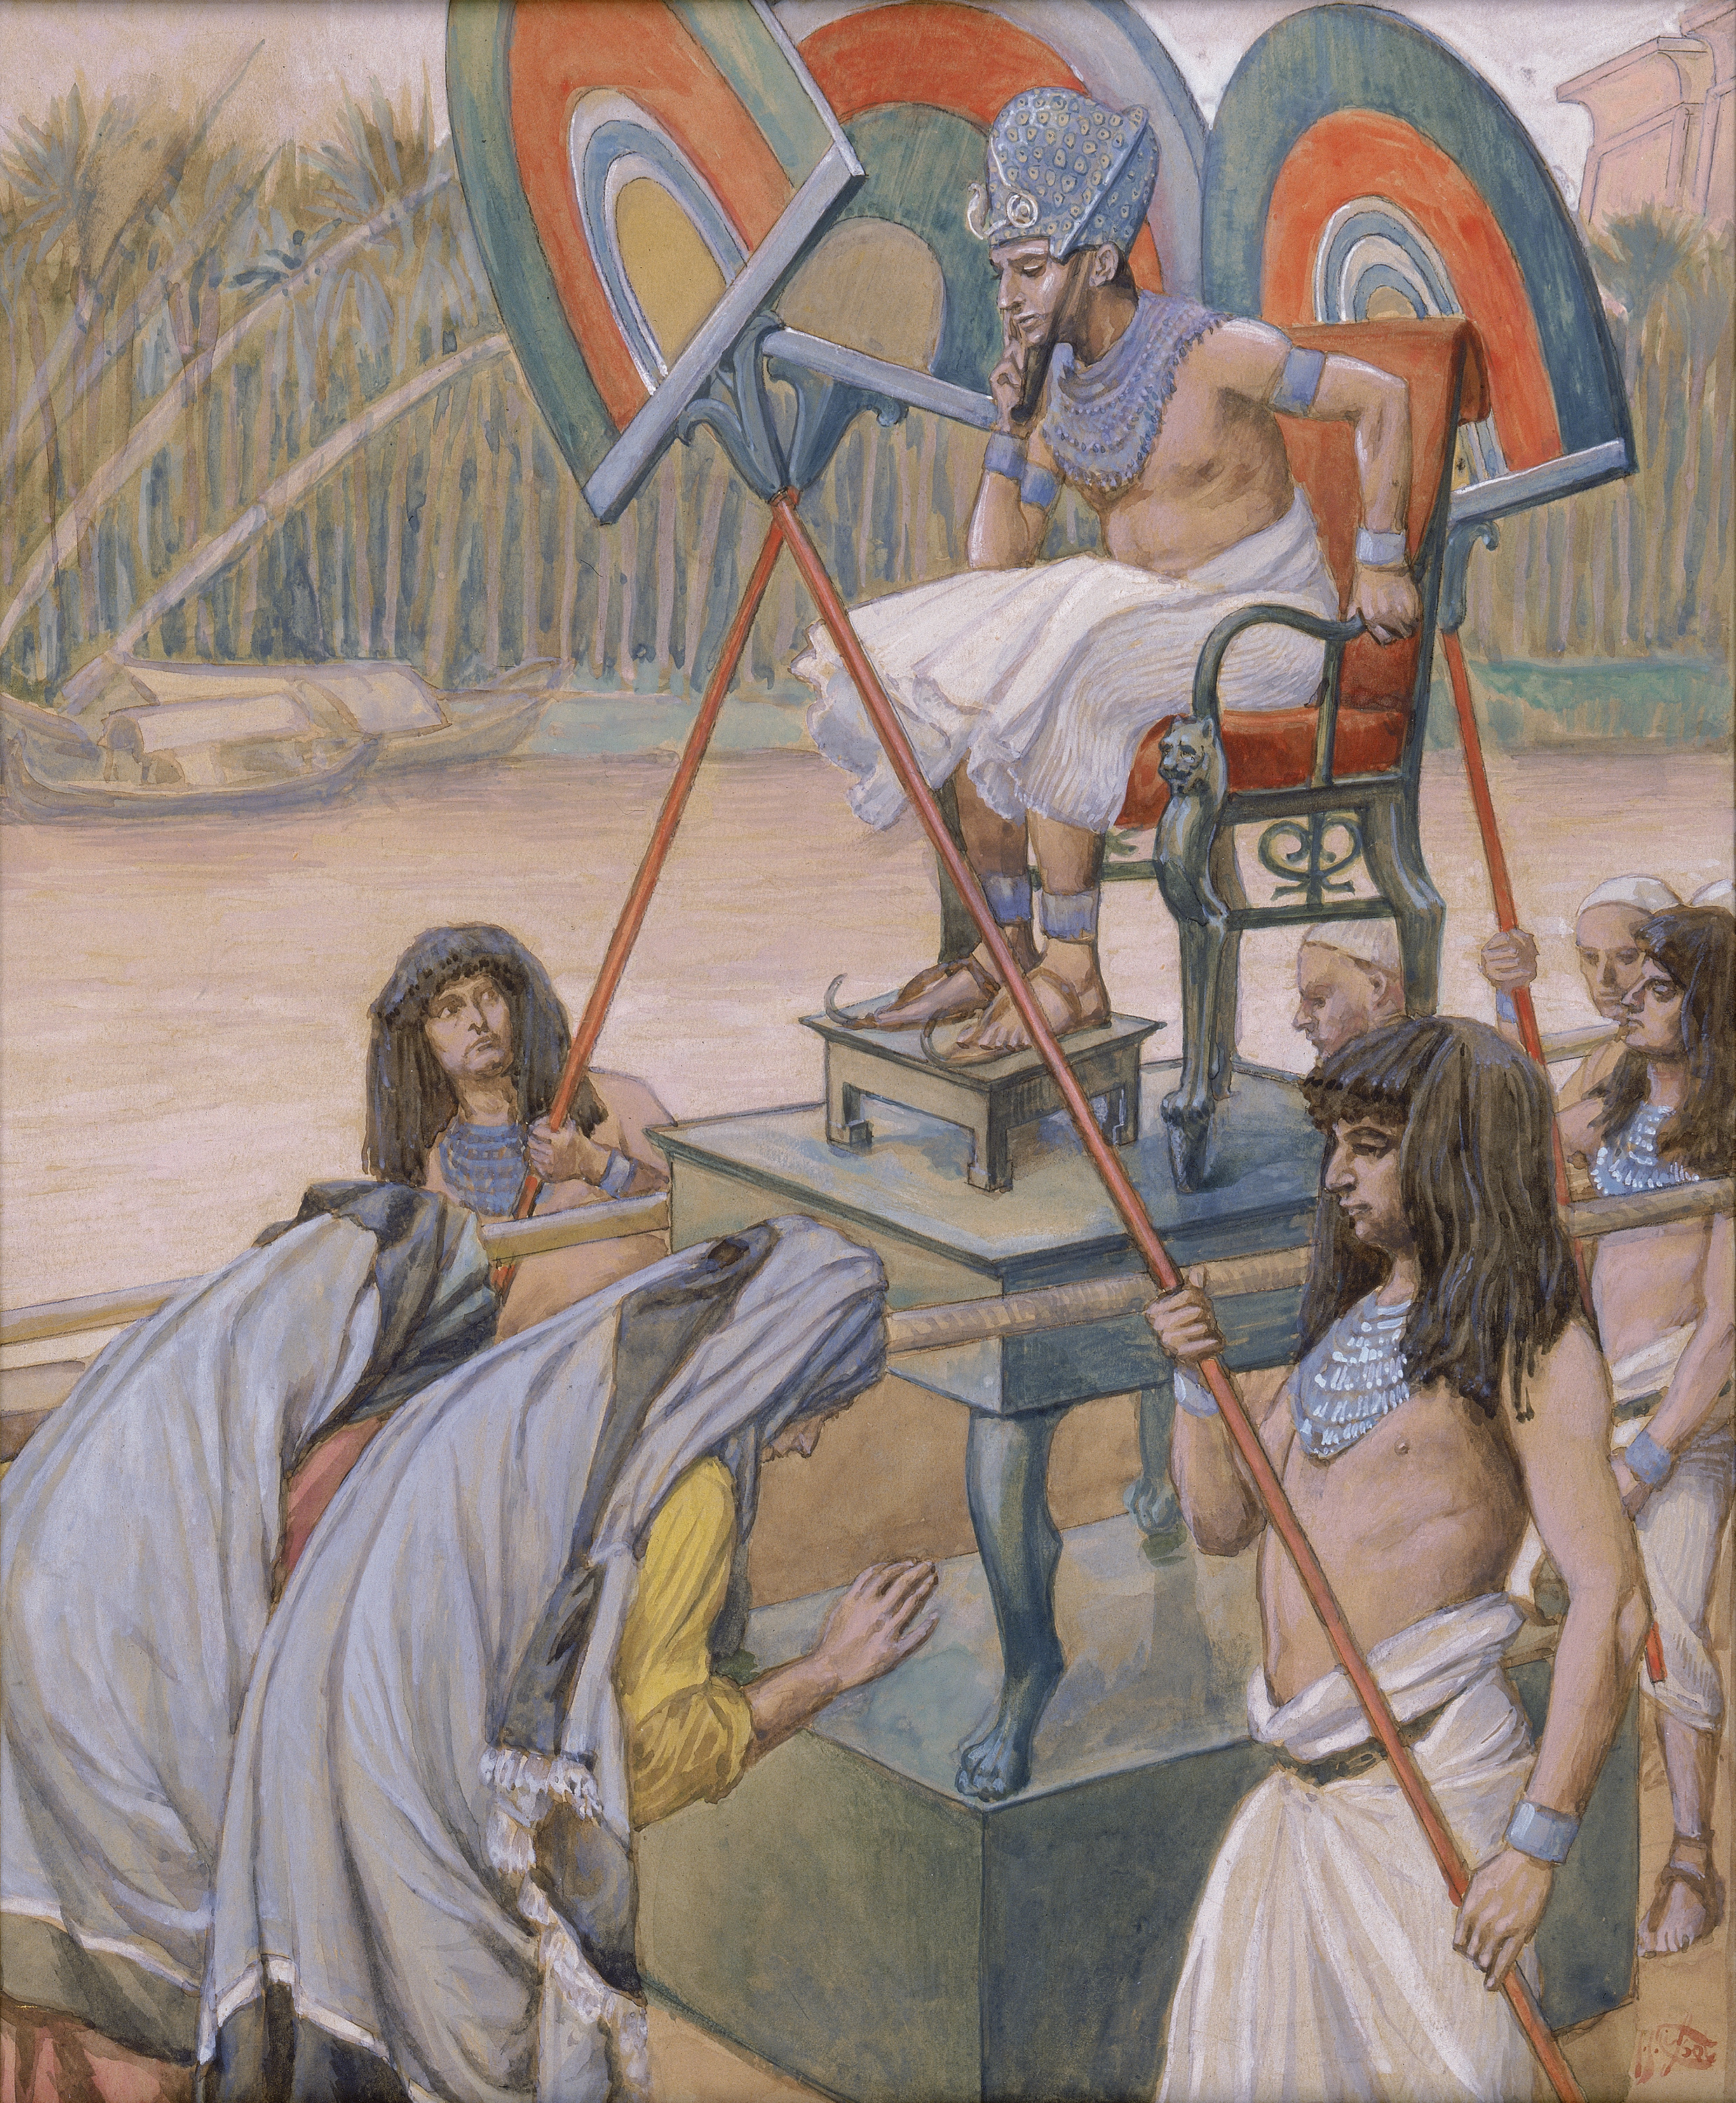
\includegraphics[width=1.3\linewidth]{midwives}
    }
    \caption{\hspace*{4cm}Obstetricēs et Rēx}
\end{figure}

\section{CAPITULUM PRIMUM}


\marginpar{quasi: velut}[In Aegyptō] fīliī Isrāēl crēvērunt, et quasi\marginpar{germināre: emmitere germina (ea quae ex plantīs veniunt: semen, fructus, cēt.)} germinantēs multiplicātī sunt:
ac rōborātī \marginpar{rōborāre: firmāre; virēs addere}nimis, implēvērunt terram.

Surrēxit intereā rēx novus super Ægyptum, quī ignōrābat Ioseph.
Et ait ad populum suum: ``Ecce, populus fīliōrum Isrāēl multus, et fortior nōbīs est.
\marginpar{ingruere: cum vi accedere}Venīte, sapienter opprimāmus eum, nē forte multiplicētur: et sī ingruerit contrā nōs bellum, addātur inimīcīs nostrīs, expugnātisque nōbīs ēgredi\-ātur dē terrā.''\marginpar{\begin{center}
\includegraphics{tab}\\tabernaculum, -ī (n)\end{center}tabernaculum quoque significat aedificium sacrum, ad formam tabernaculī}

\marginpar{praeposuit eīs magistrōs operum: dedit magistrīs potestatem super opera fīliōrum Isrāēl}
Præposuit itaque eīs magistrōs operum, ut aff-līgerent eōs oneribus: 
ædificaveruntquē urbēs tabernāculōrum Pharaōnī, Phithom et Ramessēs.
Quantōque opprimēbant eōs, tantō magis multiplicābantur, et crēscē\-bant: 
ōderantque fīliōs Isrāēl Ægyptiī, et afflīgēbant \marginpar{illūdere: deridēre}illūdentēs eīs,
atque ad amāri\-tūdinem perdūcēbant vītam eōrum operibus dūrīs \marginpar{lutum, -ī(n): terra humida}lutī et lateris, omnīque famulātū, quō in terræ operibus premēbantur. 
Dīxit autem rēx Ægyptī \marginpar{obstetrix, -īcis(f): femina quae iuvat feminam gravidam parere} obstetrīcibus Hebræōrum, quārum ūna vocā\-bātur Sephora, altera Phu\-a, 
præcipiēns eīs: ``Quandō obstetrīcābitis Hebræās, et \marginpar{partus, -ūs (m): actus pariendi} partus tempus advēnerit: sī masculus fuerit, interficite eum: sī fēmina, \marginpar{reservāre: servāre, conservāre}reservātē.''

\marginpar{nōn fēcērunt iuxtā praeceptum regis: non parent praeceptō rēgis}\marginpar{mas, maris(m): homo (vel animal) masculinus}Timuērunt autem obstetrīcēs Deum, et nōn fēcērunt iuxtā præceptum rēgis Ægyptī, sed cōnservābant marēs. 
Quibus ad sē accersītis, rēx ait: ``Quidnam est hoc quod facere voluistis, ut puerōs servārētis?''

Quæ respondērunt: ``Nōn sunt Hebreæ sīcut Ægyptiæ mulierēs: ipsæ enim obstetrīcandī habent scientiam, et priusquam veniāmus ad eās, pariunt.''

\marginpar{cōnfortāre: fortem facere, consolārī}Bene ergō fēcit Deus obstetrīcibus: et crēvit populus, cōnfortātusque est nimis.
Et quia timuērunt obstetrīcēs Deum, ædificāvit eīs domōs.
Præcēpit ergō Pharaō omnī populō suō, dīcēns: ``Quidquid masculīnī sexūs nātum fuerit, in flūmen prōiicite: quidquid fēminīnī, reservātē.''

\pagebreak

\begin{figure}[p]
    \hspace*{-2.5cm}
    \makebox[\linewidth]{
        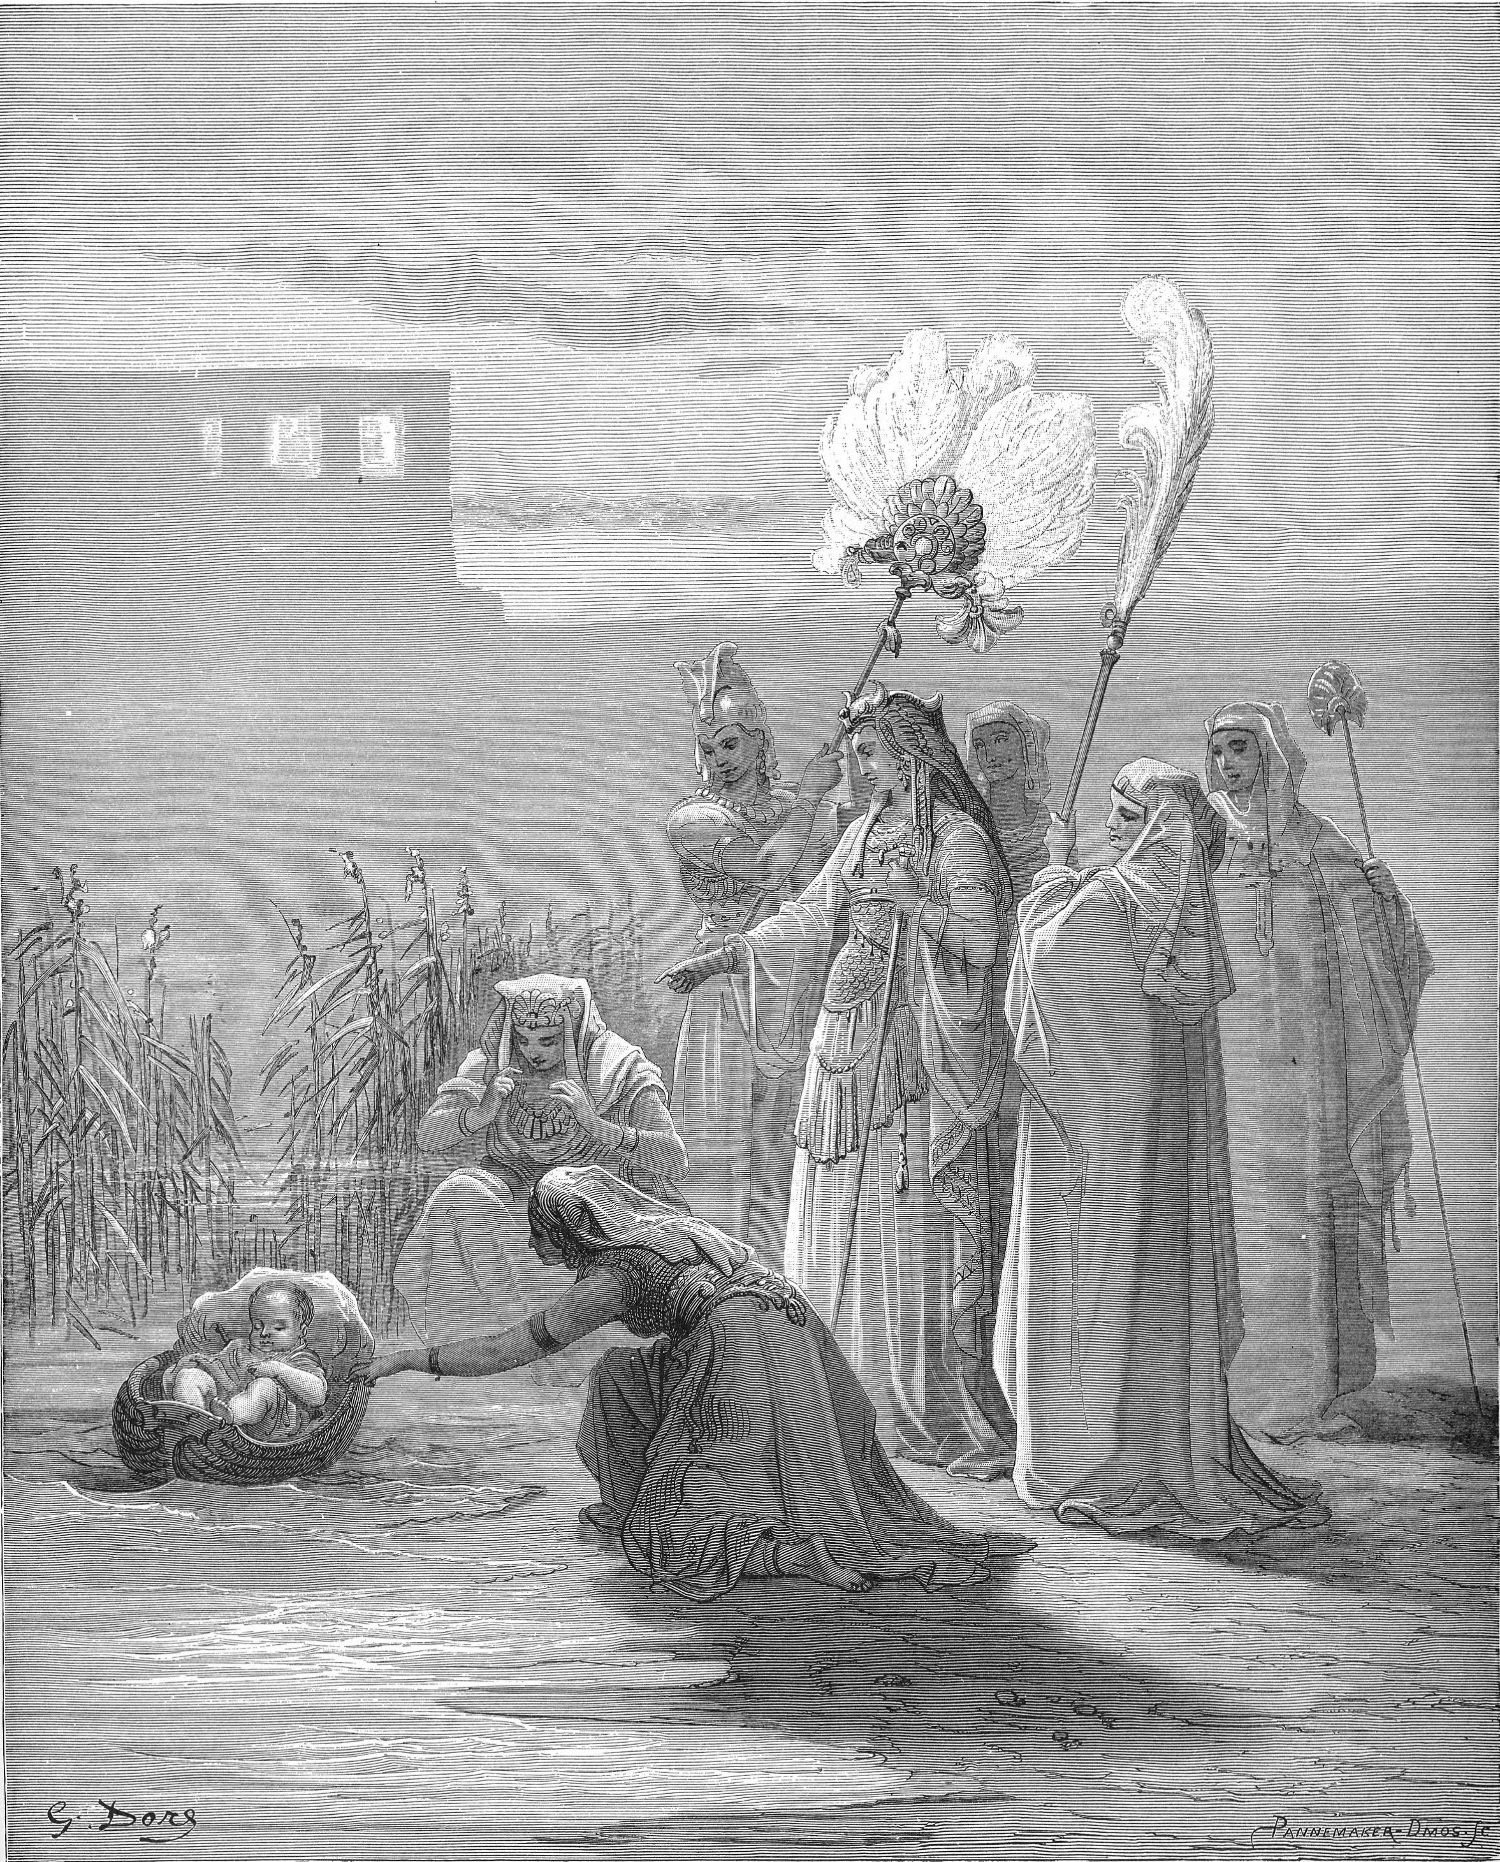
\includegraphics[width=1.3\linewidth]{babymoses.jpg}
    }
    \caption{\hspace*{-4cm}Infans Moysēs}
\end{figure}

\section{CAPITULUM SECUNDUM}

\marginpar{stirps, stirpis(m/f): stricto sensu est truncus arboris, ergo etiam origo est generis in familiis}Ēgressus est post hæc vir dē domō Levī: et accēpit uxōrem stirpis suæ.
Quæ concēpit, et peperit fīlium : et vidēns eum ēlegantem, abscondit tribus mēnsibus.
\marginpar{scirpeus/a/um: ex scirpīs factus}
\marginpar{linere: rem aliquam liquidam aut mollem alteri superinducere}
\marginpar{bitūmen, -inis(n): limus pinguis et sulphureus ē terrā emergens pluribus locīs}
\marginpar{pix, picis (f): rēs ātra quae fit ex liquōre crassō arborum coctō}
\marginpar{cārex, cāricis (f):  herba acuta et durissima, sparto similis}
\marginpar{cārectum, -ī (n): locus caricibus plenus}

\begin{figure}[hbp]
    \begin{minipage}[hbp]{0.5\linewidth}
        \centering
        
\includegraphics{fisc}
        \caption{fiscella, -ae(f)}
    \end{minipage}%
    \begin{minipage}[hbp]{0.5\linewidth}
        \centering
        
\includegraphics{brush}
        \caption{scirpus, -ī(m)}
    \end{minipage}
\end{figure}%
Cumque iam cēlāre nōn posset, sūmpsit fiscellam scirpeam,
et līnīvit eam bitūmine ac pice:
posuitque intus īnfantu\-lum, et exposuit eum in cārectō rīpæ flū\-minis,
stante procul sorōre eius, et cōnsī\-derante ēventum reī.
Ecce autem dēscendē\-bat fīlia Pharaōnis ut lavārē\-tur in flūmine.\marginpar{crepīdo, -inis (f): litus maris vel ripa fluminis, quae saxis, aut lapideo margine plerumque sternebantur}\marginpar{alveus, -ī (m): fossa, per quam fluvius defluit} Et puellæ eius gradiēbantur per crepīdinem alveī.
\marginpar{papyrio, -ōnis (m): locus papyrīs consitus}
Quæ cum vīdisset fiscellam in papȳ\-riōne,
mīsit ūnam ē famulābus suīs: et al\-lātam aperiēns,
cer\-nēnsque in eā parvulum vāgientem,
miserta eius, ait: ``Dē īnfantibus Hebræōrum est hīc.''

Cui soror puerī: ``Vīs,'' inquit, ``ut vā\-dam, et vōcem tibi mulierem hebræam,
quæ nūtr\-īre possit īnfantulum?''

Respondit: ``Vāde.''

Perrēxit puella et vocāvit mātrem suam.
Ad quam locūta fīlia Pharaōnis: ``Accipe,'' ait, ``puerum istum, et nūtrī mihi: ego dabō tibi mercēdem tuam.''

Suscēpit mulier, et nūtrīvit puerum: adultumque trādidit fīliæ Pharaōnis. 
Quem illa adoptāvit in locum fīliī,
vocāvitque nōmen eius Moysēs, dīcēns: ``Quia dē aquā tulī eum.''

In diēbus illīs postquam crēverat Moysēs, ēgressus est ad frātrēs suōs:
vīditque afflīctiōnem eōrum, et virum ægyptium percutientem quemdam dē Hebræīs frātribus suīs.
Cumque circumspexisset hūc atque illūc,
et nūllum adesse vīdisset,
\marginpar{abscondere: rem aliquam aliquo in loco ponere, ut celetur}
\marginpar{sabulum, -ī: arena}percussum Ægyptium abscondit sabulō.
\marginpar{rixāre: contendere}Et ēgressus diē alterō cōnspexit duōs Hebræōs rixantēs:
dīxitque eī quī faciēbat iniūriam: ``Quārē percutis proximum tuum?''

Quī respondit: ``Quis tē cōnstituit prīn\-cipem et iūdicem super nōs?
num occīdere mē tū vīs, sīcut heri occīdistī Ægyptium?''

Timuit Moysēs, et ait: ``Quōmodo palam factum est verbum istud?''

Audīvitque Pharaō sermōnem hunc, et quærēbat occīdere Moysēn:
quī fugiēns dē cōnspectū eius, morātus est in terrā Madiān,
\marginpar{puteus, -ī (m): aedificium (et foramen) ex quo aqua excipitur}et sēdit iuxtā puteum.
Erant autem sacerdōtī Madian septem fīliæ,
quæ vēnērunt ad hauriendam aquam:
\marginpar{adaquāre: aquam dāre}et implētīs canālibus adaquāre cupiēbant gregēs patris suī.
Supervēnēre pāstōrēs, et ēiēcērunt eās:
surrēxit\-que Moysēs, et dēfēnsīs puellīs, adaquāvit ovēs eārum. 
Quæ cum revertissent ad Raguel patrem suum, dīxit ad eās:
\marginpar{vēlox, -ōcis: celer}``Cūr vēlō\-cius vēnistis solitō?''

Respondērunt: ``Vir ægyptius līberāvit nōs dē manū pāstōrum:
\marginpar{īnsuper: praeterea}īnsu\-per et hausit aquam nōbīscum, pōtumque dedit ovibus.''

At ille: ``Ubi est?'' inquit: ``quārē dīmī\-sistis hominem? vocātē eum ut comedat pānem.''

Iūrāvit ergō Moysēs quod habitāret cum eō.
Accēpitque Sephoram fīliam eius uxōrem:
quæ peperit eī fīlium, quem vocāvit Gersam, dīcēns:
``Advena fuī in terrā aliēnā.''

Alterum vērō peperit, quem vocāvit Eliezer, dīcēns:
``Deus enim patris meī adiūtor meus ēripuit mē dē manū Pharaōnis.''

Post multum vērō tempore mortuus est rēx Ægyptī:
\marginpar{ingemīscere: dolere; prae animi angustia in sonum prorumpere et queri, suspirare}et ingemīscentēs fī\-liī Isrā\-ēl
propter opera vōciferātī sunt:
\marginpar{vōciferātus/a/um $<$ vōciferārī: vehementer exclamāre}
ascenditque clā\-mor eōrum ad Deum ab operibus.
Et audīvit gemitum eōrum,
\marginpar{pangō, pangere, pepigisse, pactum: constituere, definite statuere}ac recordātus est fœderis quod pepigit cum Abraham, Isaac et Iācōb.
Et respexit Dominus fīliōs Isrāēl et cognōvit eōs.

\end{document}
